\documentclass[12pt]{article}

\usepackage[english]{babel}
\usepackage[utf8x]{inputenc}
\usepackage{amsmath}
\usepackage{graphicx}
\usepackage[margin=1.0in]{geometry}
\usepackage{authblk}

\usepackage{fancyvrb}
\usepackage{color}
<< pygments['pastie.tex'] >>

\title{The IPython Notebook: open, reproducible scientific computing}
\author[1]{Matthias Bussonnier}
\author[2]{Jonathan Frederic}
\author[3]{Bradley M. Froehle}
\author[2]{Brian E. Granger}
\author[3]{Paul Ivanov}
\author[3]{Thomas Kluyver}
\author[3]{Fernando Perez}
\author[3]{Benjamin Ragan-Kelley}
\author[2]{Zachary Sailer}
\affil[1]{Affiliation of Matthias}
\affil[2]{Cal Poly State University}
\affil[3]{University of CA, Berkeley}

\renewcommand\Authands{ and }

\begin{document}
\maketitle

\begin{abstract}
While computing has become a foundation of all it is challenging for researchers . 
\end{abstract}

\section{Introduction}

\section{The lifecycle of research}

\section{The IPython Notebook}

\subsection{Web application}

\subsection{Notebook document format}

\subsection{Installation}

\section{Collaboration}

\section{Broader ecosystem}

\section{Future directions}

\section*{Dexy Snippets}

<% set nb = "notebooks/Chapter1_Introduction.ipynb|ipynb" %>
<% set nbdoc = nb + "" %>

The notebook \verb|<< nb >>| uses format \verb|<< d[nbdoc].nbformat >>|.

\subsection*{Markdown Content}

Here is an example of a markdown cell:

<< d['notebooks/Chapter1_Introduction--42.md'] >>

Here is the same cell in a Verbatim block:

\begin{Verbatim}
<< d['notebooks/Chapter1_Introduction--42.md'] >>
\end{Verbatim}

Here is the same cell presented as highlighted markup:

<< d['notebooks/Chapter1_Introduction--42.md|pyg|l'] >>

\subsection*{Python Content}

<< d['notebooks/Chapter1_Introduction--7-input.py|pyg|l'] >>

\begin{Verbatim}
<< d['notebooks/Chapter1_Introduction--7-output-0.txt'] >>
\end{Verbatim}

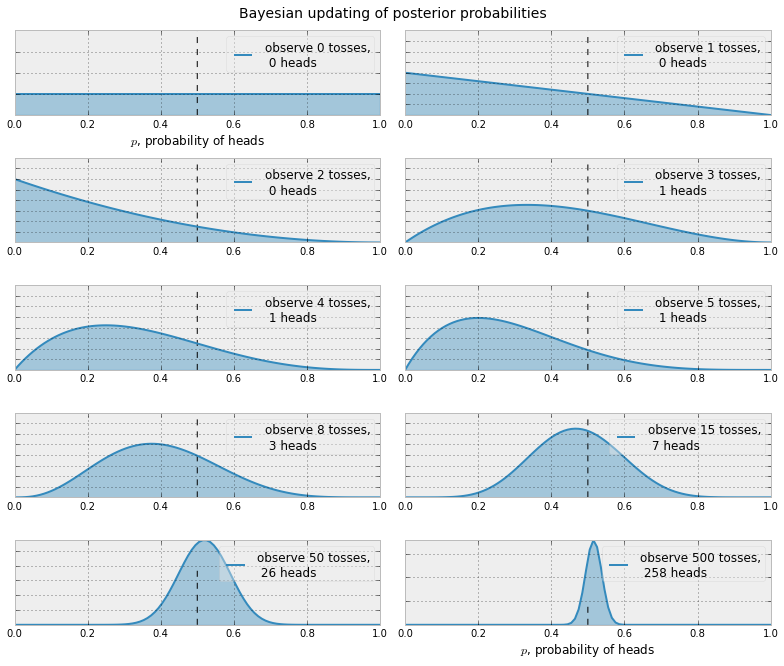
\includegraphics{notebooks/Chapter1_Introduction--7-output-1.png}

\subsection*{Iterating over Cells and Documents}

<% set cells = json.loads(d[nbdoc].cells) -%>
<% set documents = json.loads(d[nbdoc].documents) -%>

This notebook has << len(cells) >> cells and << len(documents) >> documents based on these cells.

\subsubsection*{Cells}

Here is a list of cells:

\begin{itemize}
<% for cell in cells -%>
\item{\verb|<< cell >>|}
<% endfor -%>
\end{itemize}

\subsubsection*{Documents}

Here is a list of documents:

\begin{itemize}
<% for doc in documents -%>
\item{\verb|<< doc >>|}
<% endfor -%>
\end{itemize}

Here are the contents of documents:

<% for doc in documents -%>

Here are the contents of \verb|<< doc >>|:

<% if doc.endswith(".py") or doc.endswith(".md") -%>
<< d[doc + "|pyg|l"] >>
<% elif doc.endswith(".png") -%>
\includegraphics{<< doc >>}
<% elif doc.endswith(".txt") -%>
\begin{Verbatim}
<< d[doc] >>
\end{Verbatim}
<% else -%>
Please add a display format for << doc >>.
<% endif -%>
<% endfor -%>

\end{document}
